\documentclass[12pt, a4paper]{article}

\usepackage{hyperref}
\usepackage{graphicx}
\usepackage{caption}
\usepackage{subcaption}

\title{03 Figure}
\author{Po-Hsuan Huang\\ 
    \texttt{aben20807@gmail.com}
}

\begin{document}
\vspace*{-50pt}
    {\let\newpage\relax\maketitle}

\section{figure}

Test reference: Figure~\ref{fig:example}.

\begin{figure}[ht]
    \centering
    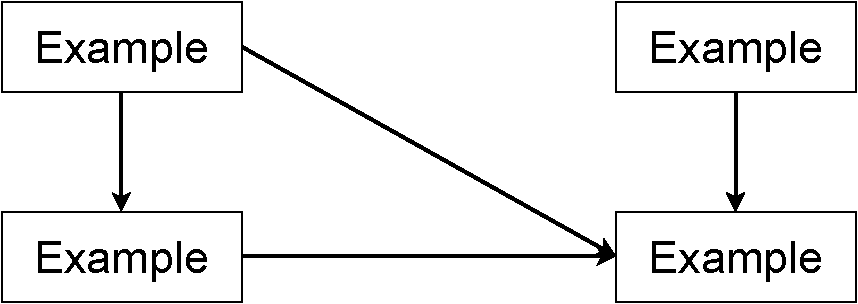
\includegraphics[width=.48\linewidth]{figures/paper-example.pdf}
    \caption{Caption for example.}\label{fig:example}
\end{figure}

\section{subfigure}

Test reference: Figure~\ref{fig:cat}.

\begin{figure}[hbt]
    \centering
    \begin{subfigure}[b]{0.48\textwidth}
        \centering
        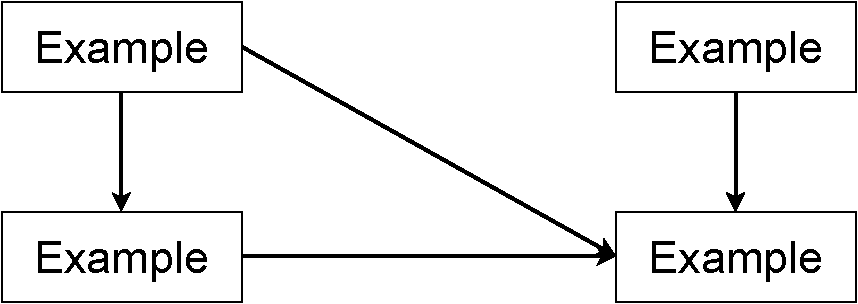
\includegraphics[width=\linewidth]{figures/paper-example.pdf}
        \captionsetup{width=.9\linewidth}
        \caption{Caption for example.}\label{fig:example2}
    \end{subfigure}
    \begin{subfigure}[b]{0.44\textwidth}
        \centering
        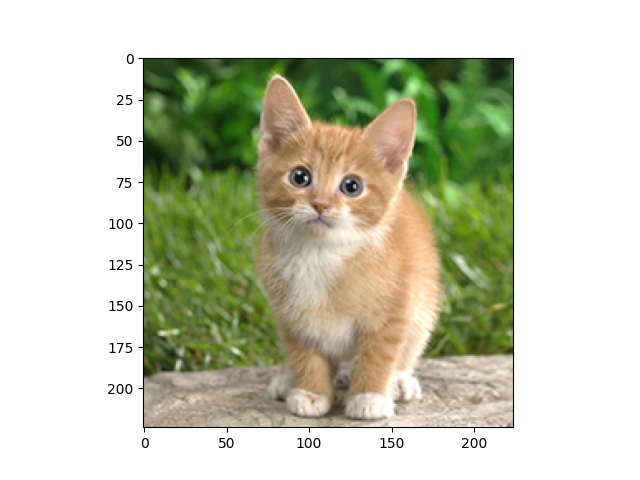
\includegraphics[width=\linewidth]{figures/cat.png}
        \captionsetup{width=.9\linewidth}
        \caption{\tiny Cat.}\label{fig:cat}
    \end{subfigure}
    \caption{Two subfigures.} \label{fig:all}
\end{figure}

\section{minipage}

\begin{table}[ht]
    \centering
    \begin{minipage}[t]{.48\linewidth}
        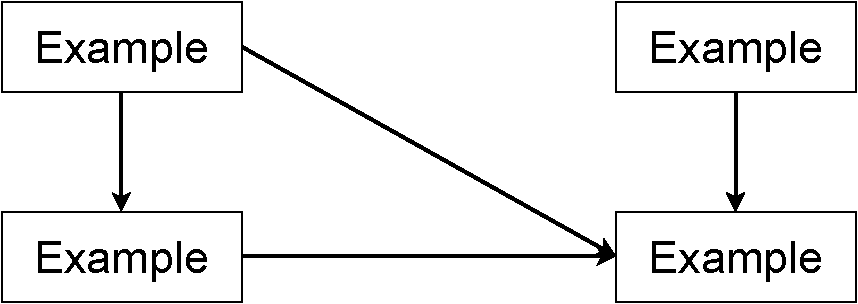
\includegraphics[width=\linewidth]{figures/paper-example.pdf}
        \captionof{figure}{First figure.}
        \label{fig:A}
    \end{minipage}
    \qquad
    \begin{minipage}[t]{.44\linewidth}
        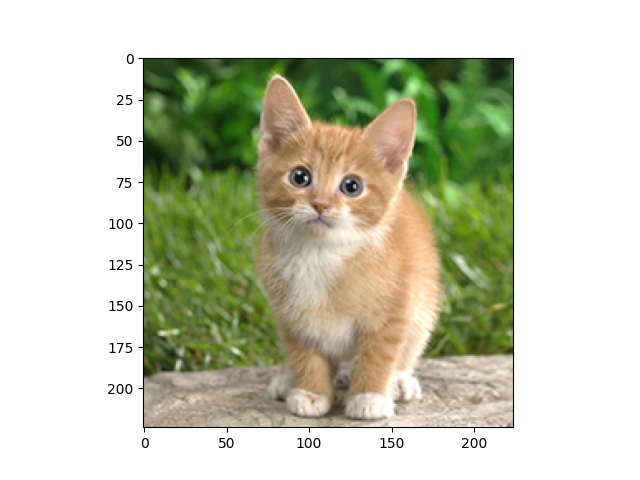
\includegraphics[width=\linewidth]{figures/cat.png}
        \captionof{figure}{Second figure.}
        \label{fig:B}
    \end{minipage}
\end{table}

\end{document}